
\setcounter{page}{2}

\section*{Flow123D}

Flow123D is simulating software based on Borland C++ Builder 6.0. It enables to solve the task of underground water flow in heterogenous rock, solute transport and their interaction with rock. Considered interaction with rock are non-equilibrium mobile-immobile pore exchange and non-linear adsorption with independent parameters in each zone (mobile/immobile) and each area (fracture/continuum rock).

The flow is based on mixed hybrid FEM. The supported task of flow are steady state flow, unsteady state flow and variable density flow. Calculation is supported on compatible or incompatible multidimenzional meshes. 

Solute transport is solved with the operator splitting.  Convection is solved with the FVM. Mobile-immobile pore exchange is solved with using analytic solution and non-linear adsorption is solved numerically.

Principle for calculation are files of mesh - \vari{msh}, material - \vari{mtr}, neighbours - \vari{ngh}, boundary conditions of flow - \vari{bcd}, eventually are needed files of boundary conditions of transport - \vari{tbc}, initial conditions of transport - \vari{tic} or initial condition of flow - \vari{fic}. Number and type of required input files are depended on the type of the problem.

File of  mesh is generated by using software \vari{GMSH}, which is distributed under the terms of the GNU GPL (www.geuz.org). File of neigbours is generated with using program \vari{NGH}. Structure of all input files are defined in the files description in detail. 

 \begin{figure}[h]
    \begin{center}
      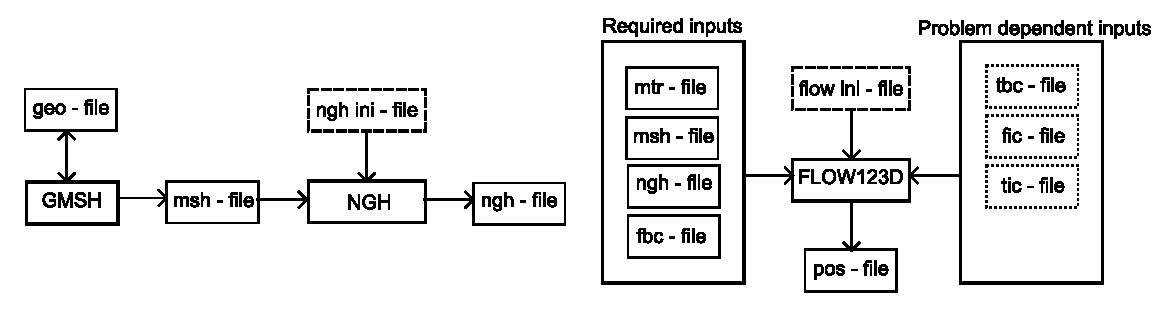
\includegraphics[scale=0.7]{schema.pdf} % 
      \caption{Scheme of calculation}
      \label{obr3}
    \end{center}
  \end{figure}

Output of the program generates \vari{pos} files supported by the \vari{GMSH}. Eventualy, it is possible using text output files for whole area, specified area or elements. 
